\documentclass[3p,twocolumn]{elsarticle}
%%\usepackage[utf8]{inputenc}
%%\usepackage[LGR,T1]{fontenc}
%%\usepackage{graphicx,amsmath}
%%\usepackage[british]{babel}
%%\usepackage[latin9]{inputenc}%SOME KIND OF CLASH WITH THIS ONE
%%\usepackage{array}
%%\usepackage{rotfloat}
%%\usepackage{textcomp}
%%\usepackage{amssymb}
%%\usepackage{amsmath} % to align equations \usepackage{mathrsfs} % curly font in math, called using mathscr
%%\usepackage{graphicx}
%%\usepackage{subcaption} % to have two images under one caption
%%\usepackage{subscript}
%%\usepackage{gensymb} %for degree symbol
\setlength{\marginparwidth}{2cm} % to set the width of the marginpar
\usepackage{todonotes}
%%\usepackage{xargs}                      % Use more than one optional parameter in a new commands
%%\renewcommand{\baselinestretch}{1.5}
\bibliographystyle{elsarticle-num}
\begin{document}
\begin{frontmatter}
\title{Advanced Characterisation of Pore Structure in Next-Generation Reactor Graphites}
\author[inst1]{Bradley Moresby-White}
\address[inst1]{University of Plymouth, Plymouth, UK}
\begin{abstract}
    
Nuclear energy accounted for 17\% of total electricity supply 
in advanced economies in 2023, avoiding the release of 72 gigatons of CO$_2$
since 1971 by replacing fossil fuel generation \cite{IEA2025NewEraNuclear}.
Maximising the operational lifespan of current and proposed nuclear reactors 
therefore reduces present and future CO$_2$ emissions.

Nuclear grade graphite is a critical component of the UK fleet of Advanced Gas
Reactors (AGRs) and those Generation IV reactors, which are graphite-moderated.
Reliable characterisation of its microporous network is therefore indispensable
for safe and optimal performance. This microstructure, in particular porosity,
dictates material properties and the evolution of those properties under
operational conditions (i.e. oxidation rates, gas diffusion, and thermal
degradation). This project develops and initially validates a methodology for
characterising the surface porosity of IG-110 and IG-430 nuclear graphites via
computational analysis of composite Scanning Electron Microscopy (SEM)
micrographs, covering an FOV (Field of View) comparable with previous Optical
Microscopy (OM) -based works (mm\(^2\) scale). A semi-automated workflow
involving composite assembly, intensity thresholding, and pore diameter
thresholding within ImageJ/Fiji was developed to quantify surface porosity and
generate void size distributions. Preliminary findings indicate that this
SEM-based approach yields statistically robust surface porosity data, capturing
features down to the micron scale. This represents a significant advancement
upon previous OM analyses of surface porosity, operating at a comparable field
of view (FOV) but now with sufficient resolution to enable reliable
classification of pores as small as 1.12 µm in diameter. The new approach
allowed for the construction of surface porosity void size distribution that
encompasses nearly the entire range of physically relevant pore sizes. The
construction of surface porosity pore size distributions over a measured size
interval down to a diameter which aligns with the steepest section of the Hg
intrusion porosimetry datasets enables validation of SEM-derived surface
porosity against experimental data. New insights are gained into the
representativeness and credibility of both this and previous OM-based works.
Initial integration of this more representative surface porosity data into a new
version of the PoreXpert void network and pore fluid simulation framework,
integrated with Hg porosimetry and N$_2$ adsorption, produced physically
plausible preliminary models of the pore network and simulated pore-fluid flow
properties such as tortuosity, diffusivity and permeability.  This enhanced
characterisation method forms a further useful methodology in refining models of
graphite behaviour, ultimately contributing to the safe and optimal operation of
current and proposed graphite-moderated nuclear reactors.\end{abstract}
\begin{keyword}keyword\sep keyword\sep keyword\end{keyword}
\end{frontmatter}

\section{Introduction}
This is a citation.\cite{JONES2020256HgHe}



\begin{figure}[ht]
    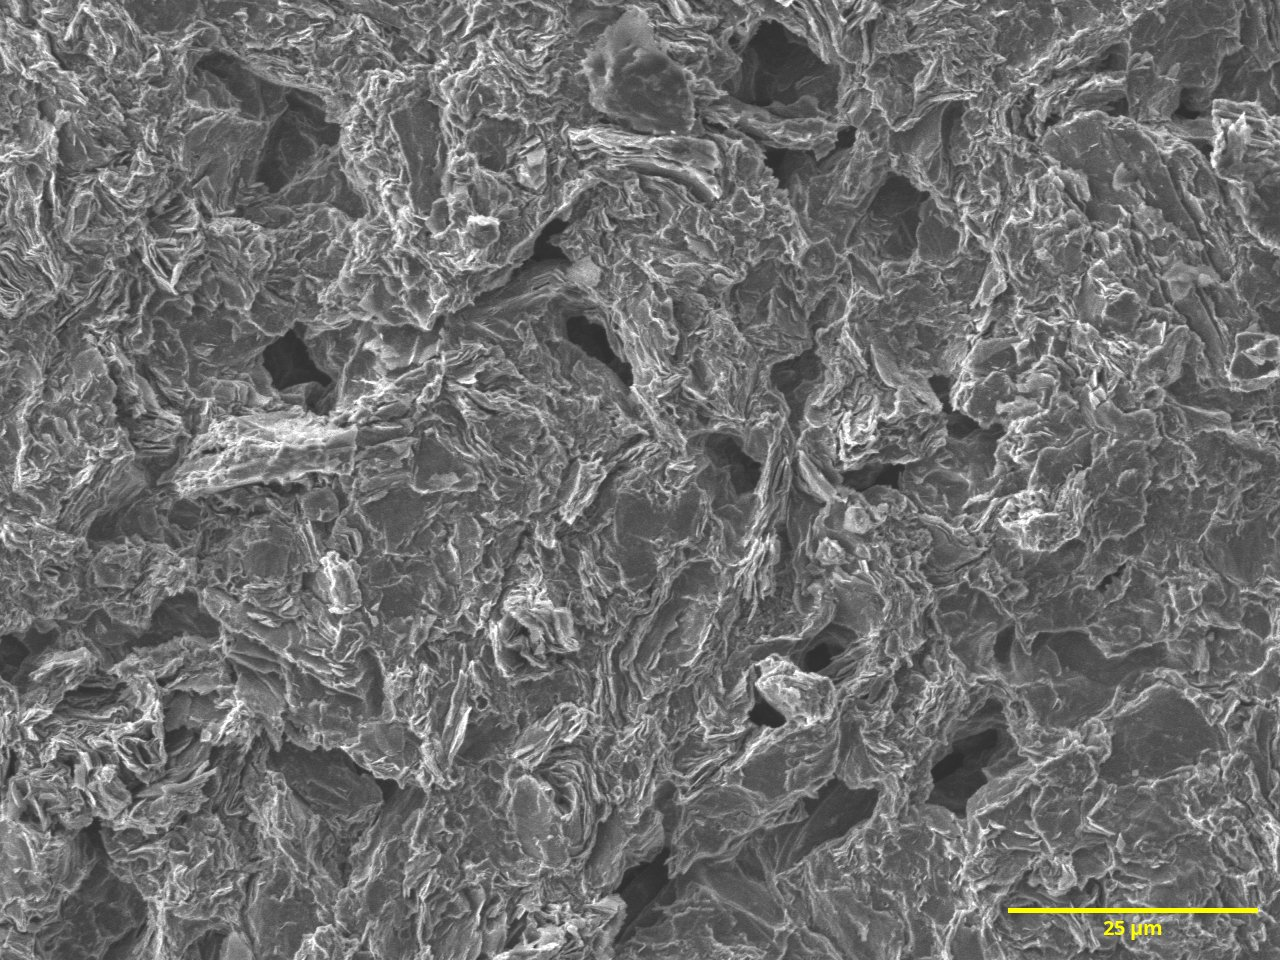
\includegraphics[width=0.45\textwidth]{./Media/image.png}
    \caption{Your caption here}
    \label{fig:testimage1}
\end{figure}
Now testing if integration between branching on VSCode and GitHub is effective.

\bibliography{bibliography}
\end{document}